\chapter{Überblick über die Hardware}
Die Hardware, die in dieser Arbeit zum Einsatz kommt, wurde eigens für den Zweck des Praktikums
''Programmierung eingebetteter Systeme'' entwickelt.

\section{Einsatz im Praktikum}
Im vorgenannten Praktikum wird den Studenten der
Umgang mit kleinen Systemen näher gebracht, die sich wesentlich von den bekannten IBM-PC-kompatiblen
Systemen unterscheiden. Das schließt die Rechenleistung, den Speicherplatz und die
Kommunikationsmöglichkeiten mit ein. 
Der Großteil der Praktikanten kennt nur das Schreiben von Programmen, die auf Betriebssystemen laufen.
Dies ist mit gewissen Vorteilen verbunden. Es gibt
Dateien, der Speicher wird verwaltet, und vieles mehr. Auf diesen kleinen Systemen, mit denen die Studenten im
Praktikum konfrontiert werden, läuft kein Betriebssystem, sondern lediglich ein Bootloader. Dieser
ermöglicht es, neue Programme auf die Platine zu laden, um diese dann ausführen zu können.
Im Laufe des Praktikums lernen die Studenten, wie man Programme in der Sprache C schreibt, und wie die Timer
sowie andere angeschlossene Geräte verwendet werden, zu denen z.B. ein LCD und ein Servomotor zählen.
Außerdem wird den Studenten vermittelt, wie der I2C-Bus funktioniert und wie man diesen benutzt.\\
Im zweiten Teil des Praktikums können die Studenten sich für ein Projekt entscheiden,
welches sie durchführen möchten (die Projektideen kommen von den Studenten).
Als Plattform für ihre Projekte wird ihnen ein Fahrzeug zur Verfügung gestellt. Dieses
Fahrzeug besitzt die aus dem ersten Teil des Praktikums bekannte Praktikumsplatine und ein WLAN-Modul,
das das Programmieren der Praktikumsplatine
ohne Kabel ermöglicht. Außerdem können hierüber Daten zwischen der Praktikumsplatine
und dem Entwicklungs-PC während
der Laufzeit ausgetauscht werden. Zusätzlich besitzt das Fahrzeug eine Motorplatine mit
zugehörigen Motoren und Rädern, die zur Fortbewegung des Fahrzeugs genutzt werden. Die
Motorplatine wird mithilfe von Befehlen, welche die Praktikumsplatine sendet, gesteuert, und
diese wiederum steuert die Motoren.\\
Die Motorplatine, für die die Betriebssoftware in der vorliegenden Arbeit entwickelt wurde, wird
im Allgemeinen von den Studenten nur benutzt, aber nicht modifiziert (auch wenn ihnen dies
freisteht). Die Leistungen, die die Motorplatine bereitstellt, 
sollen einfach anzusprechen sein, damit die Studenten sich auf das Implementieren
ihres eigenen Projektes konzentrieren können.\\
%Bild des Fahrzeugs

\section{Die Motorplatine}
Die Motorplatine wurde im Zuge der Studienarbeit von Timo Klingeberg \cite{STUD_TIMO}
entwickelt.
\begin{figure}[htb]
 \centering
 \scalebox{0.5}{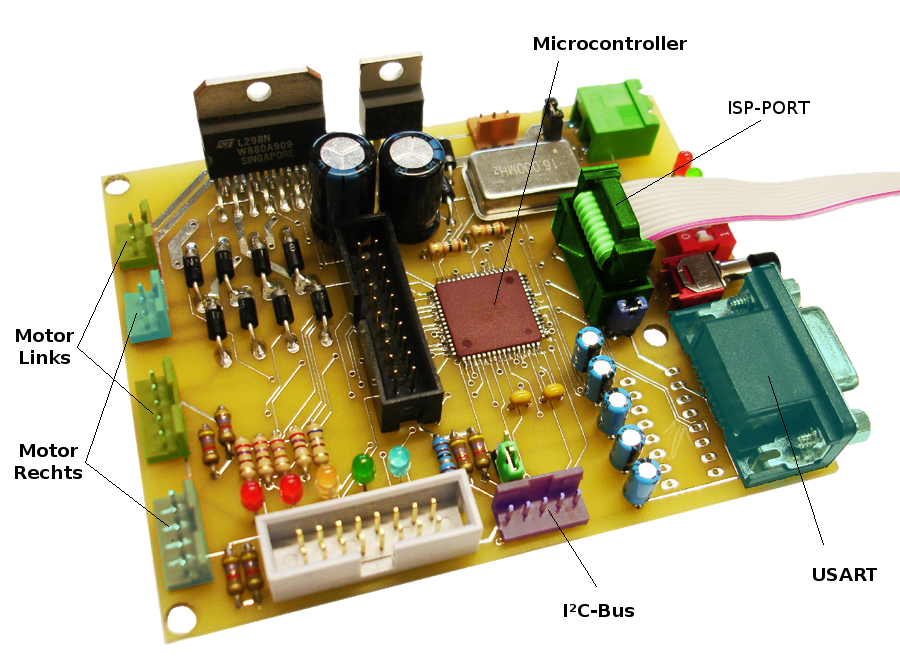
\includegraphics{pictures/board.png}}
 \caption{\label{board}Die Motorplatine}
\end{figure}
\subsection{Mikrocontroller}
Das Herzstück der Platine bildet ein Mikrocontroller der Firma Atmel.
Es handelt sich hierbei um einen ATMEGA2561\cite{ATMEGA_MANUAL}, der 256-KiB-Speicher für
Programme (Flash) hat, sowie 8-KiB-Speicher für Variablen (SRAM). Der maximale Takt für
diesen Mikrocontroller liegt bei 16 MHz, der auch ausgenutzt wird. Das bedeutet, dass
ein Takt 62,5 ns benötigt. Da der Großteil der Instruktionen des Mikrocontrollers nur
einen Takt benötigt, kann dieser theoretisch 16 MIPS leisten. Durch die Benutzung
von Funktionen, Pin-IO und bedingten Sprüngen bleibt dies aber nur eine theoretische Zahl.
Vorteilhafterweise unterstützt der Controller das ISP (In-System-Programming). Das war bei der
Entwicklung der Betriebssoftware von großem Nutzen, da hierdurch schnell und relativ
unkompliziert neue Versionen auf die Platine überspielt werden konnten.\\
Der Controller verfügt über 6 Timer. Zwei von diesen haben nur 8 Bits, die anderen vier
16 Bits. Das entspricht bei dem gegebenen Takt von 16 MHz einem maximalen Timer-Intervall von 262 ms.
Zusätzlich kann der Controller sechs Pulsweitenmodulationen betreiben, von
denen zwei für die Servomotoren genutzt werden, die die Räder antreiben.
\subsection{Ein-/Ausgabemöglichkeiten zur Praktikumsplatine}
Die Motorplatine verfügt sowohl über einen UART-Port, als auch einen I2C-Bus \cite{I2C_WIKI}, über die
die Praktikumsplatine mit der Motorplatine kommunizieren kann. Der UART-Port kann außerdem
für die Ausgabe von Debug-Informationen benutzt werden, wenn diese aktiviert wird. Im Allgemeinen
wird allerdings nur der I2C-Bus zur Kommunikation zwischen den beiden Platinen verwendet.
Da der Mikrocontroller über eingebaute Hardwarelogiken für den I2C-Bus und auch
den UART-Port verfügt, hält sich der administrative Aufwand für die Kommunikation in engen
Grenzen. Es müssen lediglich Interrupt-Service-Routinen (ISR) für diese Kommunikations-Einrichtungen zur Verfügung gestellt
werden. Dadurch ist es möglich, schnell auf Situationen zu reagieren, ohne Informationen verlieren zu können.
\subsection{Ein-/Ausgabe-Ports}
Zusätzlich zu den externen Kommunikationsmöglichkeiten mit der Praktikumsplatine besitzt der ATMEGA2561 54
programmierbare IO-Kanäle, die in Ports mit je 8 Kanälen zusammengefasst werden. 16 von diesen
Kanälen sind für die Steuerung der Servomotoren zuständig, die die Räder und die Hall-Sensoren betreiben.
Je ein Servomotor in Verbindung mit zwei Sensoren belegt einen Port. Der Servomotor benötigt 3 Kanäle
des Ports, und die Sensoren benötigen 5 Kanäle.
Diese Sensoren, die an den Motoren befestigt sind, lösen bei Bewegung der Räder Unterbrechungen aus.
Damit liefern sie Informationen, aus denen auf die Drehrichtung der Räder und die Strecke, die zurückgelegt wurde,
geschlossen werden kann.
Für jede Umdrehung eines Rades werden 360 Interrupts ausgelöst, d.h. für jedes Grad ein Interrupt. Je
nach Größe des Raddurchmessers ist eine Steckenauflösung von wenigen Millimetern möglich.
Durch die Rückmeldung der Sensoren ist es möglich, die Servomotoren nicht nur zu steuern, sondern zu regeln.
Zusätzlich kann die Geschwindigkeit der einzelnen Rädern aus diesen Informationen ermittelt werden.
Die Informationen werden genutzt, um die Pulsweiten-Modulation zu regeln, mit der die Servomotoren angetrieben
werden.\\
Neben diesen zwei Ports zum Regeln der Motoren sind weitere zwei Ports nach außen gelegt. Mithilfe
der Pins dieser zwei nicht belegten Ports konnte eine weitgehend unverfälschte Untersuchung des
Echtzeitverhaltens der Betriebssoftware durchgeführt werden.

\subsection{LCD}
Die Motorplatine verfügt über einen Anschluss für ein LCD. Dieses LCD kann zur autonomen Ausgabe
von Informationen genutzt werden. Die Betriebssoftware nutzt diese Möglichkeit,
wenn ein LCD angeschlossen ist, und der zugehörige DIP-Schalter aktiviert wurde.
Es werden die aktuelle Version der Betriebssoftware, die Optionen und, falls vorhanden,
der aktuelle Befehl in hexadezimaler Darstellung ausgegeben. Zu den Optionen zählen der Status der Debug-Ausgaben,
welche Kommunikations-Einrichtung verwendet wird, und der Zustand des ABS. Diese Optionen
werden groß geschrieben, wenn sie aktiviert sind, und klein geschrieben, wenn sie
deaktiviert sind. Die Betriebssoftware ist auf LCDs eingestellt, die 4 Zeilen und 20 Zeichen je Zeile besitzen.
Sollte ein anderes LCD angeschlossen werden, ist eine korrekte Ausgabe, ohne
Änderungen an der Software, nicht möglich.
